%%%%%%%%%%%%%%%%%%%%%%%%%%%%%%%%%%%%%%%%%%%%%%%%%%%%%%%%%%%%%%%%%%%%%%%%%%%%%%%%%%%%%%%%%%%%%%%%%%%%%%%%%%%%%%%%%%%%%%%%%%%%%%%%%%%%%%%%%%%%%%%%%%%%%%%%%%%
% This is just an example/guide for you to refer to when submitting manuscripts to Frontiers, it is not mandatory to use Frontiers .cls files nor frontiers.tex  %
% This will only generate the Manuscript, the final article will be typeset by Frontiers after acceptance.   
%                                              %
%                                                                                                                                                         %
% When submitting your files, remember to upload this *tex file, the pdf generated with it, the *bib file (if bibliography is not within the *tex) and all the figures.
%%%%%%%%%%%%%%%%%%%%%%%%%%%%%%%%%%%%%%%%%%%%%%%%%%%%%%%%%%%%%%%%%%%%%%%%%%%%%%%%%%%%%%%%%%%%%%%%%%%%%%%%%%%%%%%%%%%%%%%%%%%%%%%%%%%%%%%%%%%%%%%%%%%%%%%%%%%

%%% Version 3.4 Generated 2018/06/15 %%%
%%% You will need to have the following packages installed: datetime, fmtcount, etoolbox, fcprefix, which are normally inlcuded in WinEdt. %%%
%%% In http://www.ctan.org/ you can find the packages and how to install them, if necessary. %%%
%%%  NB logo1.jpg is required in the path in order to correctly compile front page header %%%

\documentclass[utf8]{frontiersSCNS} % for Science, Engineering and Humanities and Social Sciences articles
%\documentclass[utf8]{frontiersHLTH} % for Health articles
%\documentclass[utf8]{frontiersFPHY} % for Physics and Applied Mathematics and Statistics articles

%\setcitestyle{square} % for Physics and Applied Mathematics and Statistics articles
\usepackage{url,hyperref,lineno,microtype,subcaption}
\usepackage[onehalfspacing]{setspace}

\linenumbers


% Leave a blank line between paragraphs instead of using \\


\def\keyFont{\fontsize{8}{11}\helveticabold }
\def\firstAuthorLast{Albishry {et~al.}} %use et al only if is more than 1 author
\def\Authors{Nabeel Albishry\,$^{1}$, Tom Crick\,$^{2,*}$ and Theo Tryfonas\,$^{3}$}
% Affiliations should be keyed to the author's name with superscript numbers and be listed as follows: Laboratory, Institute, Department, Organization, City, State abbreviation (USA, Canada, Australia), and Country (without detailed address information such as city zip codes or street names).
% If one of the authors has a change of address, list the new address below the correspondence details using a superscript symbol and use the same symbol to indicate the author in the author list.
\def\Address{$^{1}$Faculty of Computing \& IT, King Abdulaziz University, Jeddah, Saudi Arabia\\
$^{2}$Department of Computer Science, Swansea University, Swansea, UK\\
$^{2}$Faculty of Engineering, University of Bristol, Bristol, UK}
% The Corresponding Author should be marked with an asterisk
% Provide the exact contact address (this time including street name and city zip code) and email of the corresponding author
\def\corrAuthor{Corresponding Author}

\def\corrEmail{thomas.crick@swansea.ac.uk}




\begin{document}
\onecolumn
\firstpage{1}

\title[Chains and Trees: Topical Patterns in Twitter Trends]{Chains and Trees: Topical Patterns in Twitter Trends} 

\author[\firstAuthorLast ]{\Authors} %This field will be automatically populated
\address{} %This field will be automatically populated
\correspondance{} %This field will be automatically populated

\extraAuth{}% If there are more than 1 corresponding author, comment this line and uncomment the next one.
%\extraAuth{corresponding Author2 \\ Laboratory X2, Institute X2, Department X2, Organization X2, Street X2, City X2 , State XX2 (only USA, Canada and Australia), Zip Code2, X2 Country X2, email2@uni2.edu}


\maketitle


\begin{abstract}

%%% Leave the Abstract empty if your article does not require one, please see the Summary Table for full details.
\section{}
% For full guidelines regarding your manuscript please refer to \href{http://www.frontiersin.org/about/AuthorGuidelines}{Author Guidelines}.

% As a primary goal, the abstract should render the general significance and conceptual advance of the work clearly accessible to a broad readership. References should not be cited in the abstract. Leave the Abstract empty if your article does not require one, please see \href{http://www.frontiersin.org/about/AuthorGuidelines#SummaryTable}{Summary Table} for details according to article type. 

With thousands of topics -- in multiple languages -- trending on Twitter across the world every day, it is increasingly challenging to provide in-depth analysis of current issues, topics and themes being discussed across these various locations and jurisdictions. Utilising a graph structure approach, this paper presents an exploration of topical patterns of trends on Twitter across various regions to provide simple and extensible approaches to allow deeper insight and analysis into these trends and how they propagate across locales. It is based on a year-long data collection ({\emph{N}}=2,307,163) and analysis between 2016-2017 of seven Middle Eastern countries (Bahrain, Egypt, Kuwait, Lebanon, Qatar, Saudi Arabia, and the United Arab Emirates). Using this year-long dataset, the project identified two interesting structures of topics, based around chains and trees. Trend topics that manifested themselves in these structures are found to represent key emerging concerns and interests to users on the relevant platform.

\tiny
 \keyFont{ \section{Keywords:} trends, topic structures, topic-trees, topic-chains, network graphs, Twitter} %All article types: you may provide up to 8 keywords; at least 5 are mandatory.
\end{abstract}

\section{Introduction}\label{intro}

With c.500 million tweets per day of user-generated content on Twitter, trending topics serve as valuable sources of information on highlighting what is going on in the world, or in specific locations. Apart from the ``official'' trend lists provided by the platform, generating insight from trends and topics detection has been receiving increasing attention from across a variety of big social data-driven research domains. In health for example, monitoring and analysis of trending topics on social media has been adopted to measure emerging public health issues, such as the spread of influenza~\cite{Achrekar2011,Parker2015}. Furthermore, across the marketing and business domains, topic detection and classification are valuable approaches to extract knowledge and insight on public opinions from posts on social media~\cite{blamey-et-al-2012,blamey-et-al-2013,Bello2013,mostafa-et-al-ai2016,albishry-et-al:ssei2018}, including analysing political view of users and voting intentions~\cite{oatley+crick:2014,Fang2015}.

The impact of live trending data on public opinion and perceptions has transformed social media campaigns and public relations strategy. This has made trends a valuable target for manipulation~\cite{Zhang2017}, stuffing~\cite{Irani2010}, spamming~\cite{Sedhai2015,Chu2012}, and hijacking~\cite{VanDam2016}. Interestingly, deeper analysis of trend hijacking cases suggests that increasing social media engagement may not always be beneficial for public relations strategies~\cite{Sanderson2016,albishry-et-al:ssei2018}.

Clustering and classification of trending topics based on content are common approaches in analysing Twitter trends~\cite{Zubiaga2011,Benhardus2013,Ferragina2015,albishry-et-al:iccci2017}. Content-independent methods to model trends progression through the dynamics of users interactions have been successful previously~\cite{TenThij2016}; other studies have also attempted to provide real-time classification or detection of trends~\cite{Mathioudakis2010,Zubiaga2015}. With the increasing demand for trends analysis across various domains, customisable clustering tools that can be used by non-technical users have started to emerge~\cite{Arn2018}.

\section{Methodology}\label{method}

The approach in this study consists of two main parts; graph construction and text analysis. First, the {\emph{weighted base graph}} is constructed to capture raw trends data in the form of country-trend relationships. Trend texts are then used to generate ngrams, with the {\emph{derived graph}} generated from these trend-ngram relationships. The different parts of these two graphs are then merged to link countries to topics of interests.

\subsection{Locales}

Seven Middle Eastern countries were selected for this study: Bahrain, Egypt, Kuwait, Lebanon, Qatar, Saudi Arabia, and the United Arab Emirates (UAE). The selection includes countries with relatively large population (e.g. Egypt: 97,553,000) and relatively small populations (e.g. Bahrain: 1,493,000)~\cite{UnitedNationsDepartmentofEconomicandSocialAffairs2017}. Kuwait is reported to have the most active daily users on Twitter~\cite{Salem2017}; as of March 2016, Saudi Arabia and Egypt generated 33\% and 20\% of the tweets in the Middle Eastern region. Bahrain is the most balanced location in terms of gender breakdown of active users. Interestingly, between March 2014 and March 2016, Lebanon was the only location in the Middle Eastern states that has not seen growth in active users, while UAE increased by 60\%. The Gulf Cooperation Council countries -- Bahrain, Kuwait, Qatar, UAE, and Saudi Arabia -- were reported to have the highest penetration rates~\cite{Salem2017}.

\subsection{Data Collection}

Trending topic lists in the seven countries were monitored for a year between October 2016 and October 2017. Every hour, trending lists were collected through the Twitter REST API, which resulted in 7,948 hour's worth of records for all the countries, totalling 2,307,163 trend records. It is important to note that the Twitter API does not necessarily provide trends data for every request; for example, it is possible to receive no information for tweet volume. For each location, the list of available trending topic is returned. From this list, two pieces of information are extracted from each trend record; {\emph{woeid}}: the Yahoo! Where On Earth ID (WOEID) of the location; {\emph{name}}: text of trending topic (e.g `{\texttt{\#Call\_For\_Action}}').

While the Twitter API returns a list of trending topics for a specific {\emph{woeid}} location, the tweet volumes do not provide a comprehensive measure of the tweeting activity in that location. Rather, the tweet volume refers to the overall number of tweets containing the trend, regardless of their location. Although the Twitter documentation\footnote{\url{https://developer.twitter.com/en/docs/trends/trends-for-location/api-reference/get-trends-place}} does not provide the necessary depth of detail on this, it was apparent after observing trends that showed up in various locations. Trends were found with the same tweet volume across all locations and, hence, participation volume of each location was not possible to be accurately measured. Therefore, the context of this study does not include any reference to this volume entity.

\subsection{Base Graph Construction: Temporal edges}

This directed graph was constructed from raw data. The main use of this graph was to measure the temporal appearance order of the trends for places. As the graph was aimed to mainly capture data structures, constructing this graph was a simple process.  In this graph each edge had a timestamp of the trend appearance, therefore the connected pair of nodes might possess more than one edge, as shown in Figure~\ref{fig:basegraph}. The participation of the country measures the number of trends it generates, hence, two types of nodes were included in this graph: country and trend. It is important to note that the network was constructed whereby the edges originated from the country node toward the trend node. Although an undirected graph could be used, the direction orientation was important for distinguishing the node types by their indegrees. The nodes with a zero indegree identified countries, while the indegree of the trends nodes could not be less than one. Changing the direction of the edge would provide the same results, and in this case, inverted centrality measures were used. For example, the indegree was used instead of the outdegree, and vice versa.

\begin{figure}[htb] \centering
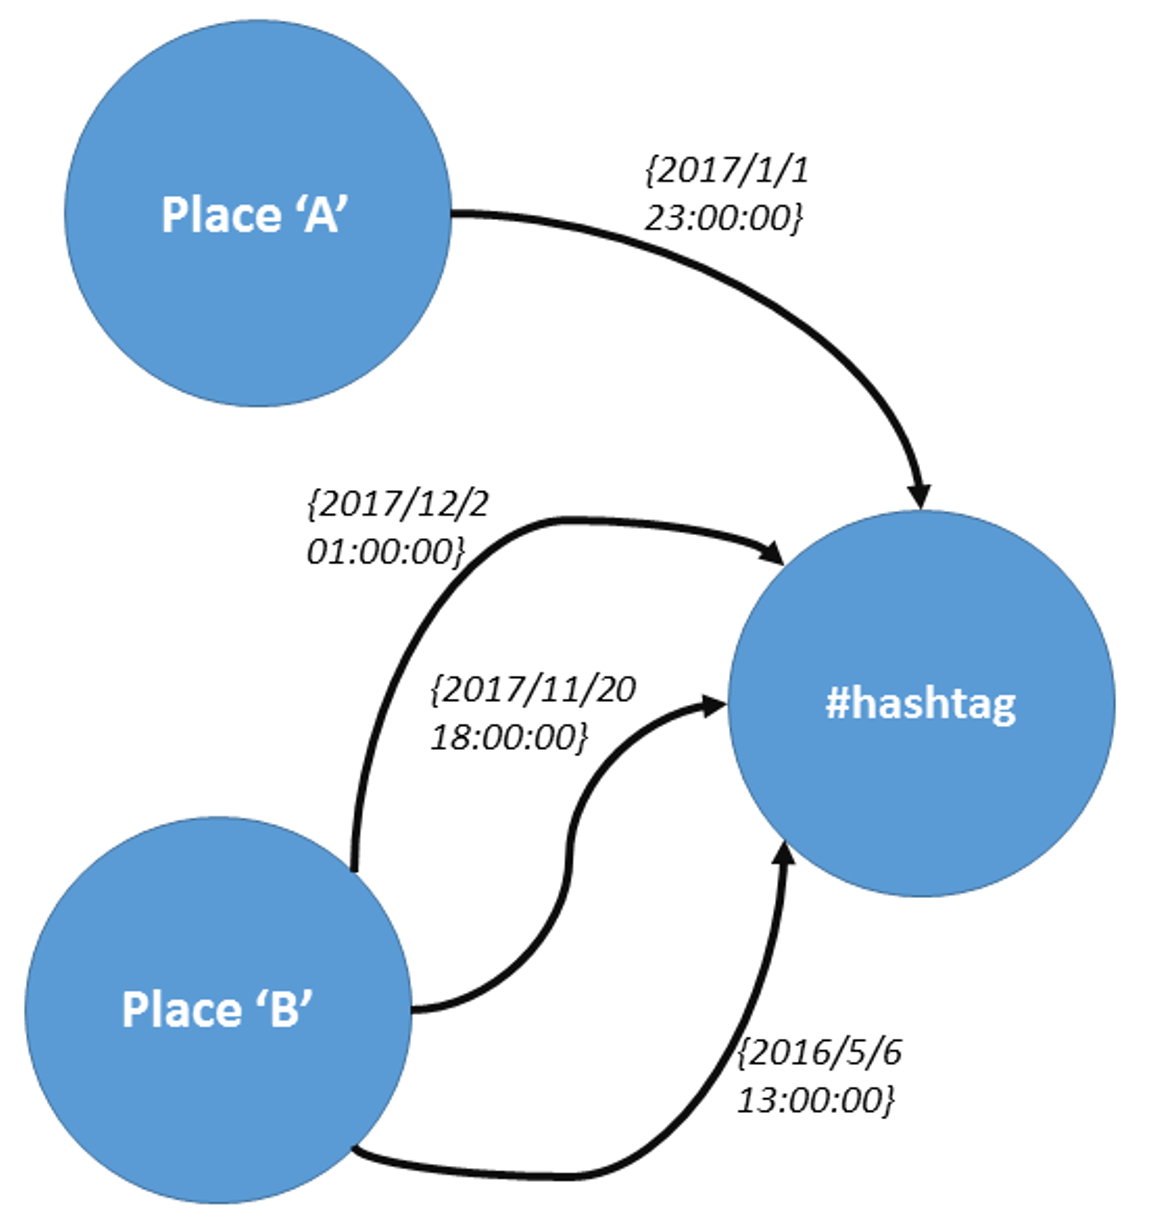
\includegraphics[width=\columnwidth]{images/base_graph.png}
\caption{Illustration of the base graph}
\label{fig:basegraph}
\end{figure}


\subsection{Derived Graph Construction: Weighted edges}

This graph is generated from the base graph, following the algorithm shown in Table~\ref{tbl:algorithm1}. It is a directed graph and that consists of two trend entities: {\emph{place}} and {\emph{trend}}. Nodes represent places and trends, and are linked with {\emph{weighted}} edges. The feature of weighted edges in this graph is used to measure the popularity of trends, repetition rate, participation of countries, and the volume of the engagement. Figure~\ref{fig:w_graph} shows an example of such graph.


\begin{table}
\centering
\begin{tabular}{l|l}
\hline
{\emph{1}} & weighted\_graph = empty\_graph()\\
{\emph{2}} & \textbf{FOR} edge \textbf{IN} base\_graph.edges():\\
{\emph{3}} &  $\>\>\>\>$\textbf{IF} weighted\_graph.has\_edge(country, trend):\\
{\emph{4}} &  $\>\>\>\>\>\>\>\>$ edge\_weight+=1\\
{\emph{5}} &  $\>\>\>\>$\textbf{ELSE:}\\
{\emph{6}} &  $\>\>\>\>\>\>\>\>$ add\_edge(country, trend)\\
\hline
\end{tabular}
\caption{Trend-Ngram graph construction algorithm}
\label{tbl:algorithm1}
\end{table}


%\begin{figure}[htb] \centering
%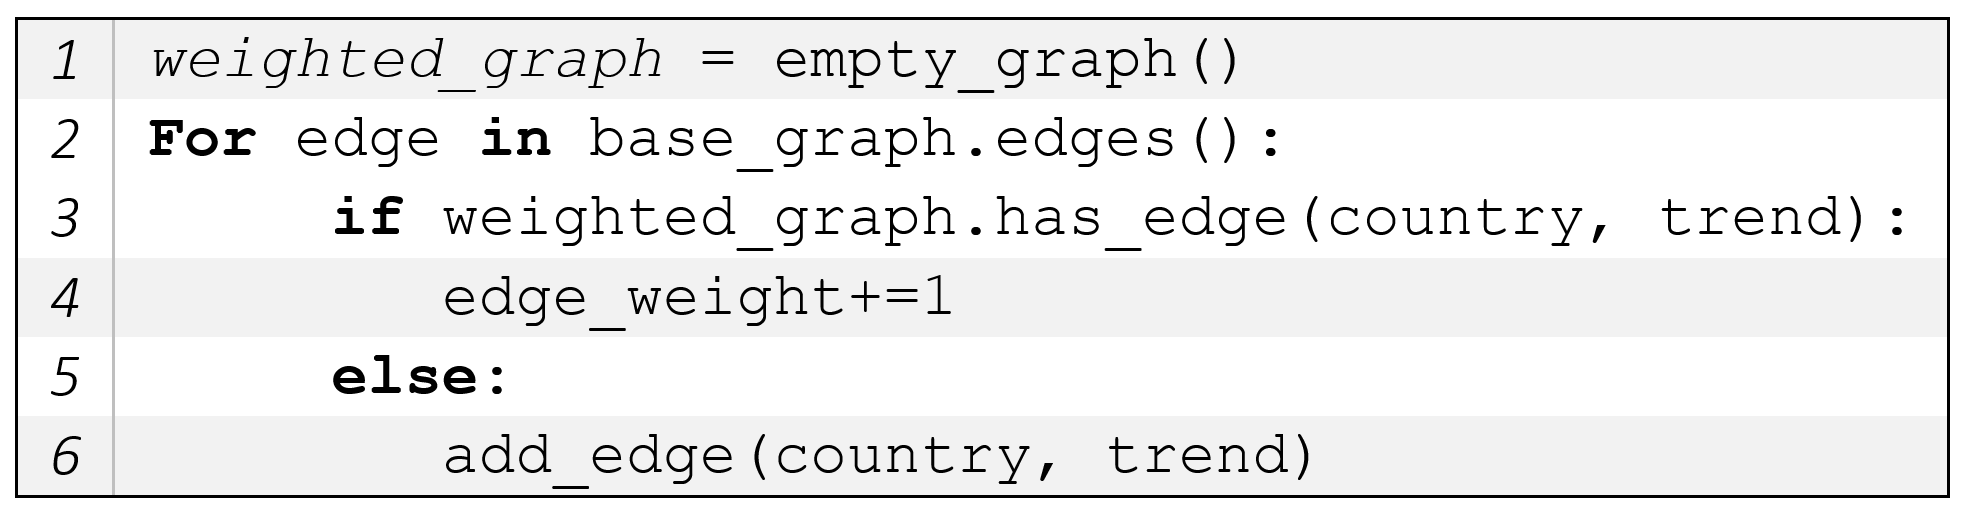
\includegraphics[width=\columnwidth]{images/algorithm1.png}
%\caption{Country-Trend weighted graph construction algorithm}
%\label{fig:algorithm1}
%\end{figure}


\begin{figure}[!ht] \centering
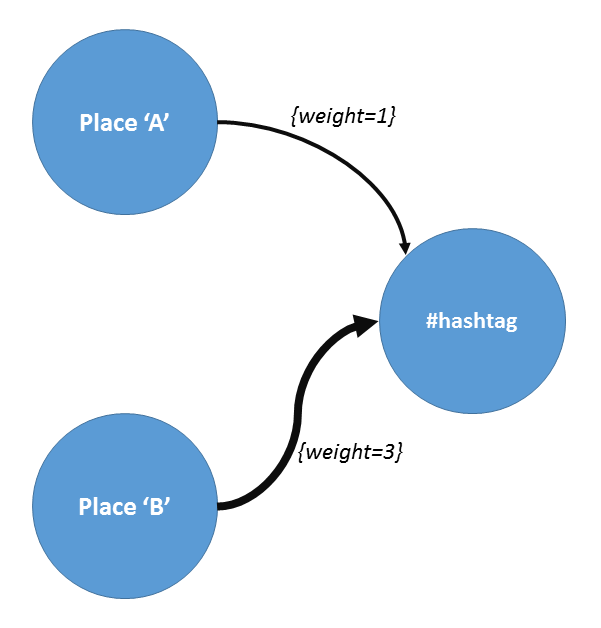
\includegraphics[width=\columnwidth]{images/w_graph.png}
\caption{Example of weighted graph}
\label{fig:w_graph}
\end{figure}


\subsection{Text analysis and Ngraming}

Trends exist in the form of phrases or hashtags. The main textual difference between these is that hashtags appear as a connected chain of characters with no whitespaces, while trending phrases include spaces. To create a hashtag with more than one word, it must be possible to distinguish the words while maintaining their connectivity, and Twitter allows underscores to be used in multiple word hashtags. For languages such as English, letter capitalisation is an additional popular option in social media for hashtagging, such as {\texttt{\#ThisIsAnExample}}. However, languages such as Arabic, Urdu, and Farsi, do not employ capitalisation in the same way, therefore the only means of separating words is to use underscores.

The textual analysis in this study required the trend texts to be tokenised to generate ngrams. This process was straightforward for the phrase trends, although the hashtag trends included a number of variations that required consideration during the textual processing. In capitalised English hashtags, for example, it was unclear whether the capital letters referred to the beginning of words or abbreviations. In contrast, Arabic hashtags use underscores to separate words, which therefore make word separation an easy and accurate task to accomplish. As the sample countries were from the Arab region, it was anticipated that most tweeting activity would occur in the Arabic language, since an earlier study demonstrated that 72\% of all tweets in the Arab region are in Arabic~\cite{Salem2017}.

In this present study, the textual analysis accounted for underscores and spaces only where they occurred as word separators. While this implied that capitalised hashtags should be considered as a single word, this would not provide an accurate analysis for this group of trends, but since Arabic trends were dominant in the dataset, and only capitalised hashtags were affected, this was not anticipated to have an impact on the results of the analysis.


\subsection{Derived Graph: Trend-Ngrams}

This directed graph utilised the trend nodes in the base graph to generate its nodes and edges. It included two types of nodes: trend and ngram. To generate ngrams from a trend, the trend first required tokenisation. The trends displayed in two forms, either as a phrase, such as `coffee international day', or a hashtag such as `{\texttt{\#coffee\_international\_day}}'.  Phrase trends can be tokenised from their original form, while hashtags do not include spaces, and hence appear as one word, and therefore first required processing in order that all of the trends were translated into phrase form before being tokenised. The hashtags processing involved stripping them of the `{\texttt{\#}}' sign, and replacing the underscores with spaces. Then, preserving the word order, the phrases were tokenised, and all possible ngrams then generated.  The original trend was connected to all of the ngrams generated, and an additional length attribute was added to each node within the graph, as shown in lines five and seven in Table~\ref{tbl:algorithm2}.  This attribute was used later in the analysis and the visualisation setting. Applying this algorithm to the hashtag '{\texttt{\#coffee\_international\_day}}' resulted in the graph shown in Figure~\ref{fig:tngraph}.

\begin{table}
\centering
\begin{tabular}{l|l}
\hline
{\emph{1}} & trend\_ngram\_graph = empty\_graph()\\
{\emph{2}} & \textbf{FOR} node \textbf{IN} base\_graph.nodes():\\
{\emph{3}} &  $\>\>\>\>$ \textbf{IF} indegree(node) != 0:\\
{\emph{4}} &  $\>\>\>\>\>\>\>\>$tokens = tokenise(node)\\
{\emph{5}} &  $\>\>\>\>\>\>\>\>$trend\_ngram\_graph.add\_node(node, length(tokens))\\
{\emph{6}} &  $\>\>\>\>\>\>\>\>$\textbf{FOR} n \textbf{IN} all\_ngrams(tokens):\\
{\emph{7}} &  $\>\>\>\>\>\>\>\>\>\>\>\>$ trend\_ngram\_graph.add\_node(n, length(n)):\\
{\emph{8}} &  $\>\>\>\>\>\>\>\>\>\>\>\>$ \textbf{IF} trend\_ngram\_graph.has\_edge(node, n):\\
{\emph{9}} &  $\>\>\>\>\>\>\>\>\>\>\>\>\>\>\>\>$ edge\_weight += 1\\
{\emph{10}} & $\>\>\>\>\>\>\>\>\>\>\>\>$ \textbf{ELSE:}\\
{\emph{11}} & $\>\>\>\>\>\>\>\>\>\>\>\>\>\>\>\>$ add\_edge(node, n)\\
\hline
\end{tabular}
\caption{Trend-Ngram graph construction algorithm}
\label{tbl:algorithm2}
\end{table}

% \begin{figure}[htb] \centering
% 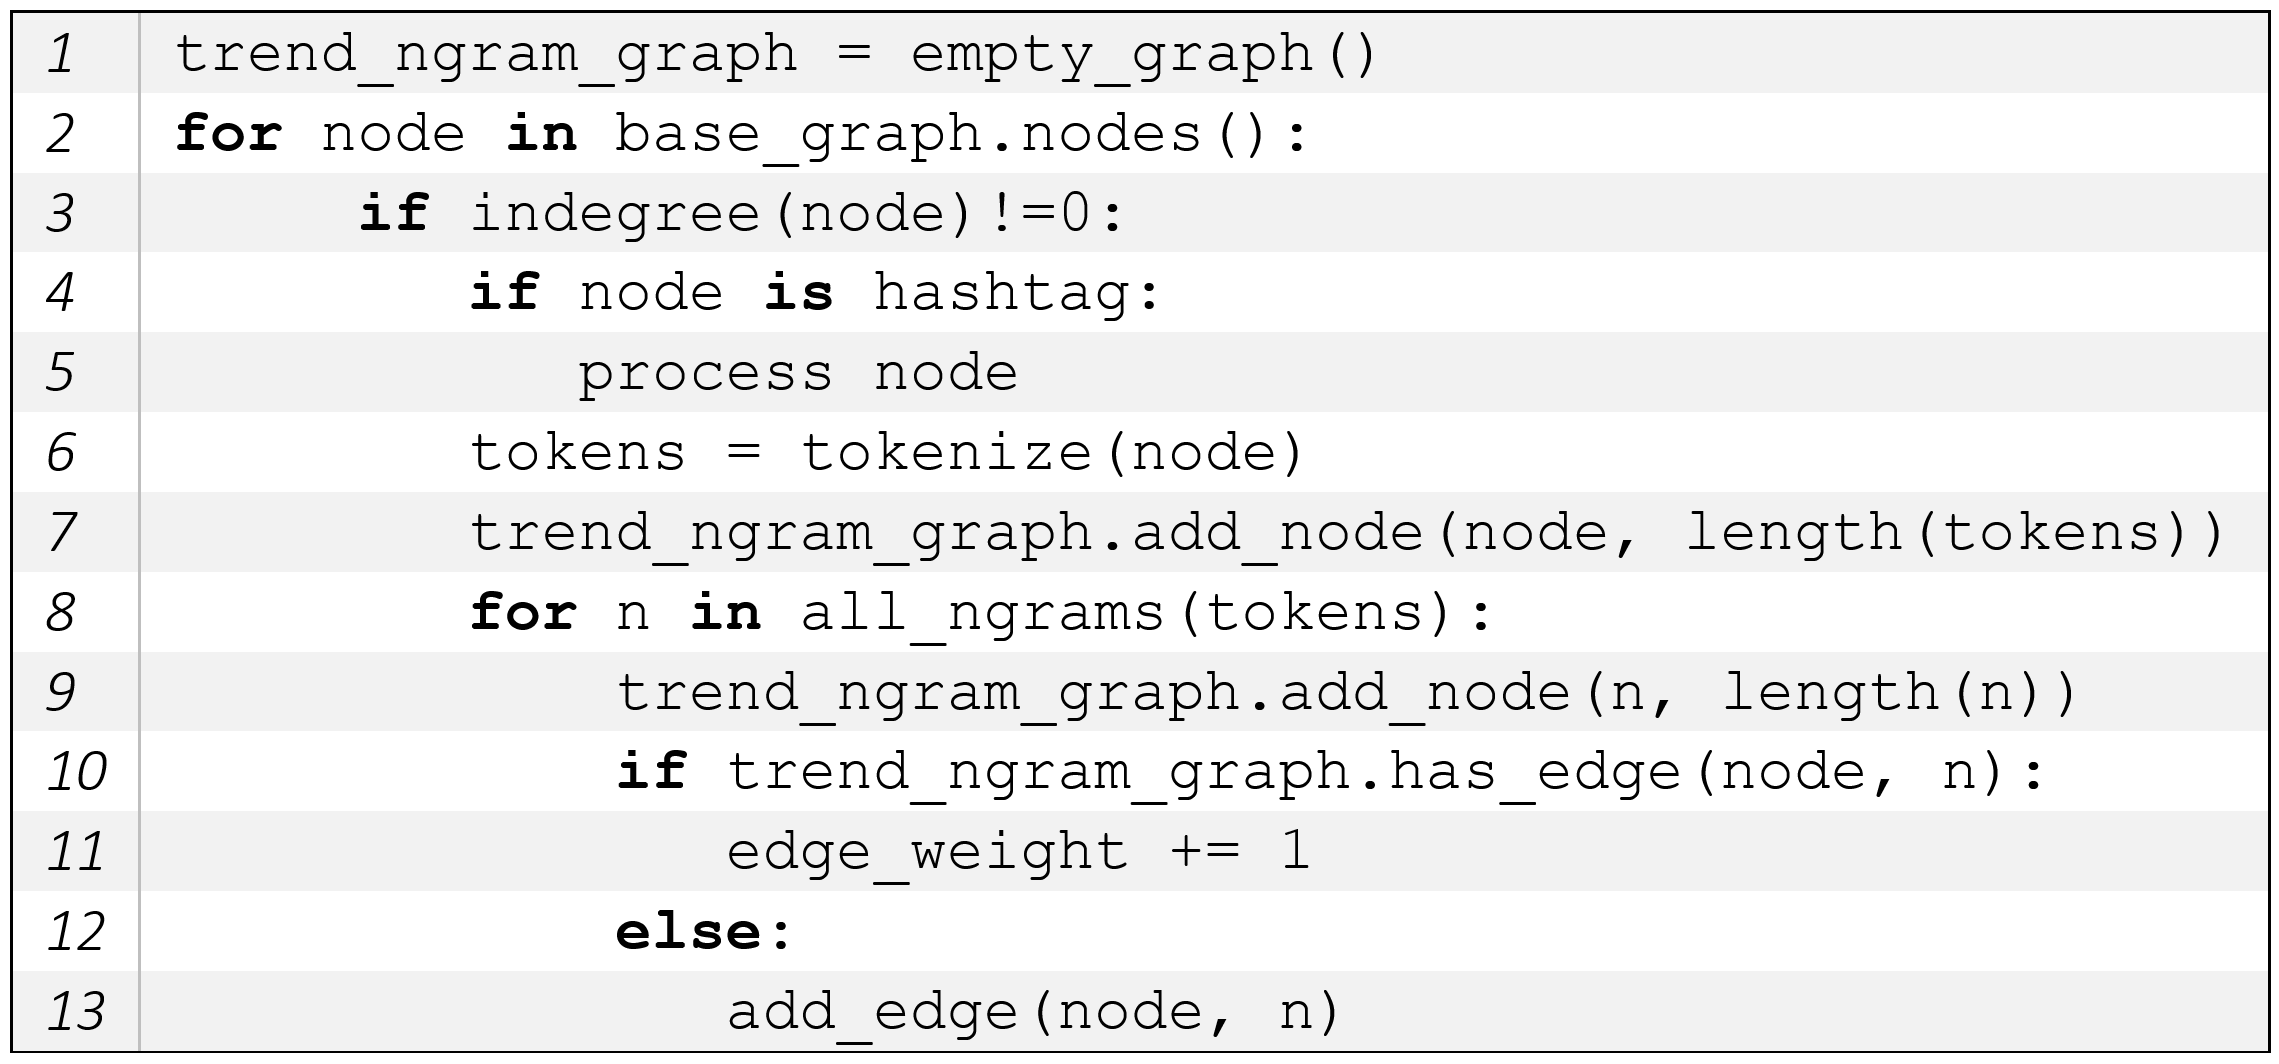
\includegraphics[width=\columnwidth]{images/algorithm2.png}
% \caption{Trend-Ngram graph construction algorithm}
% \label{fig:algorithm2}
% \end{figure}

\begin{figure}[!tb] \centering
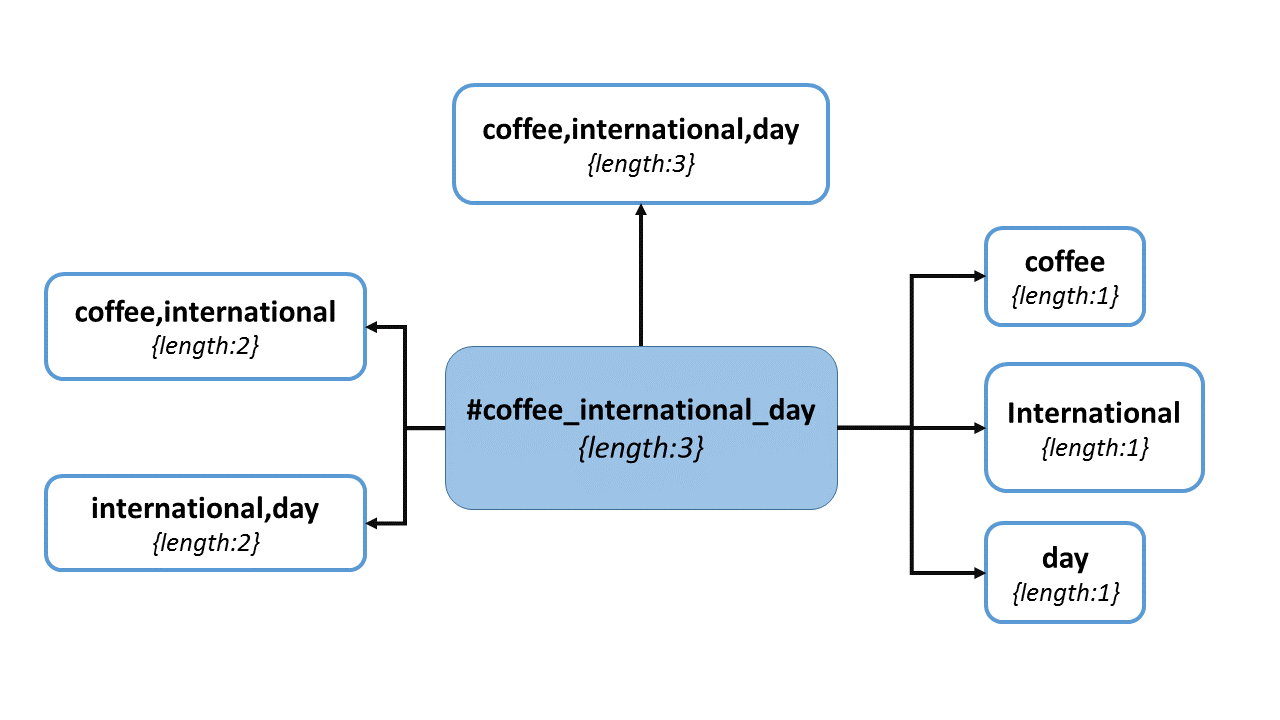
\includegraphics[width=\columnwidth]{images/trend_ngram_example.png}
\caption{Trend-Ngram graph example}
\label{fig:tngraph}
\end{figure}

A trend node in the base graph cannot be repeated. Therefore, the edges linking the trend to the ngrams in this graph were expected to have a fixed weight of 1.  However, observation of the edge weights revealed edges with higher weights, namely 2 and 3, occurring in trends with repeated words, such as `{\texttt{\#welcome\_you\_welcome}}'.  In total, 264 trends had two repeated words, while five trends had three. Since this small number of cases fell outside the context of this study, and the analysis of this graph did not utilize individual edge weights, they did not affect the results. As a result, only the indegree and outdegree centrality measures were employed for this graph, with both the indegree of all of the trend nodes, and the outdegree of the ngram nodes being 0. These two measures were employed in the analysis phase to distinguish the node types. Furthermore, the indegree of the ngram nodes reflected the number of the connected trend, and was at least 1. The outdegree of the trend nodes indicated the number of related ngrams. As the ngrams were generated from the trends, the outdegree of the trend was found to be fixed, and was equivalent to $(n(n+1))/2$, where n is length of trend.

\section{Results}\label{results}

Observation of the weighted graph provided an overall evaluation of activity for trends and places. In total there were 76,266 distinct trends that trended 2,307,163 times across all locations; this suggests that trends may appear repeatedly over time. The overall repetition ratio in the dataset was 97\%, and ranged from 80\% to 98\% for individual locations, with Saudi Arabia scoring lowest and Qatar scoring highest rate. {\emph{Indegree}}, {\emph{outdegree}}, and {\emph{edges}} were used to conduct subsequent results, with further explanation to follow in the relevant sections.

\subsection{Textual features of trends}

As can be seen in Figure~\ref{fig:trends_lengths_wind}, two-word trends were the most common trends. Presence of 1 and 3-word trends were at similar level, and 4-word trend are a little lower. Then, lengths started to show dramatic drop from 5-word onwards. Additionally, weighted indegree of trend was found strongly correlated with the word length.

\begin{figure}[htb] \centering
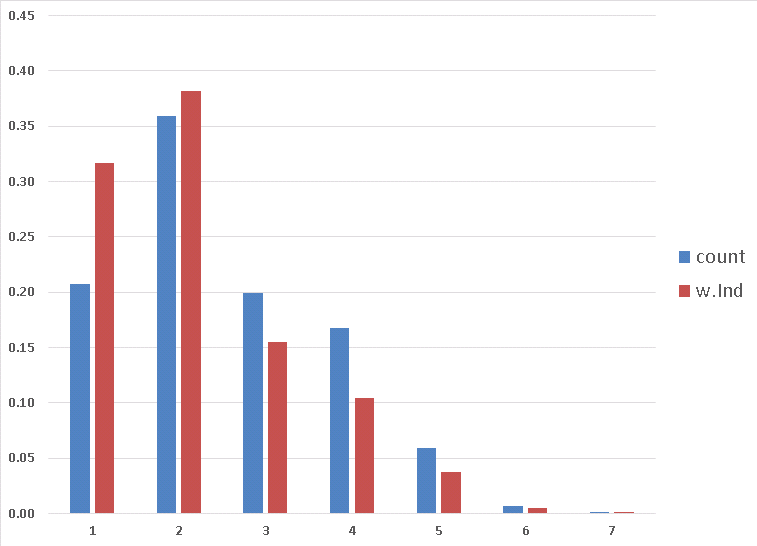
\includegraphics[width=\columnwidth]{images/trends_lengths_wind.png}
\caption{Ratios of trend lengths and their weighted indegree}
\label{fig:trends_lengths_wind}
\end{figure}

A single odd case was found in which processing the trend’s text resulted in 16 words, which indicate very unusual case. Further investigation uncovered that the trend consists of three words that were intentionally letter spaced, seemingly for fun. To clarify it further, the trend was in Arabic and it is the equivalent of {\texttt{\#WriteInSeparateLetters} but was written as {\footnotesize{{\texttt{\#w\_r\_i\_t\_e\_I\_n\_S\_e\_p\_a\_r\_a\_t\_e\_L\_e\_t\_t\_e\_r\_s}}}}. Therefore, this was removed from the dataset before progressing to further analysis. This demonstrates additional benefit of analysing length of trend in removing such odd cases.

\subsection{Chain and Tree topics}

Investigation of trend-ngram graph uncovered two special group of trends that appeared in form of trees and chains.  Each form features trends that relate to same ngram but longer by exactly one segment in terms of word numbers. This last segment is found to be the key to distinguish trend trees from chains. Last segments of all related trends are examined to confirm if they are digit or words. Then, chain likelihood is calculated by measuring the ratio of digits to words is measured.  For example, “{\texttt{\#Call\_for\_action\_1}}”, “{\texttt{\#Call\_For\_Action\_2}}”, and “{\texttt{\#Call\_for\_action\_3}}” form a trend chain and relate to the ngram “Call,For,Action”. An example of a trends tree graph would be the trends “russian\_foreign\_minister” and “american\_foreign\_minister” relating to ngram “foriegn,minister”. Indegree of the ngram indicates number of relating trends and measure length of the trend chain or number of topic branches. Having a perfect chain with high indegree is very likely to uncover well-planned ‘Twitter campaign’, regardless of its aims or representativeness of public concerns on the real world.  The example in Figure~\ref{fig:stc_chain} represents a perfect chain with bigram origin node. The example is related to a well-known boycott campaign that started early October 2016 against the Saudi Telecommunication Company (STC)~\cite{naffee-2016}.  On the other hand, when value of chain likelihood is found 0, some perfect trend trees were identified. Representation of a perfect trends tree is shown in Figure~\ref{fig:ministers_tree}.  The core of the graph is the bigram ‘foreign,minister’, and is connected to 25 trends, such as ‘saudi\_foreign\_minister’ and ‘iranian\_foreign\_minister’. As can be seen, trend trees were found featuring more general topics compared to trend chains that feature more specific topics or issues.

\begin{figure*}[htb] \centering
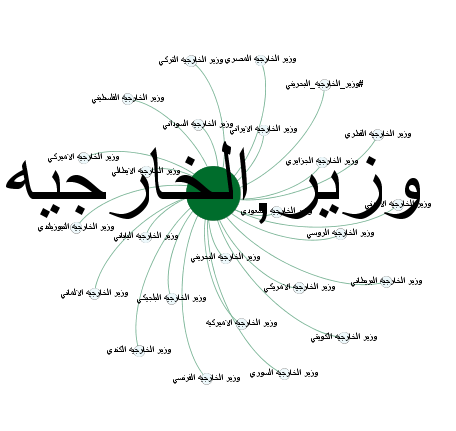
\includegraphics[width=0.7\textwidth]{images/foreign_ministers_tree.png}
\caption{Topic tree for foreign ministers trends}
\label{fig:ministers_tree}
\end{figure*}

\begin{figure*}[htb] \centering
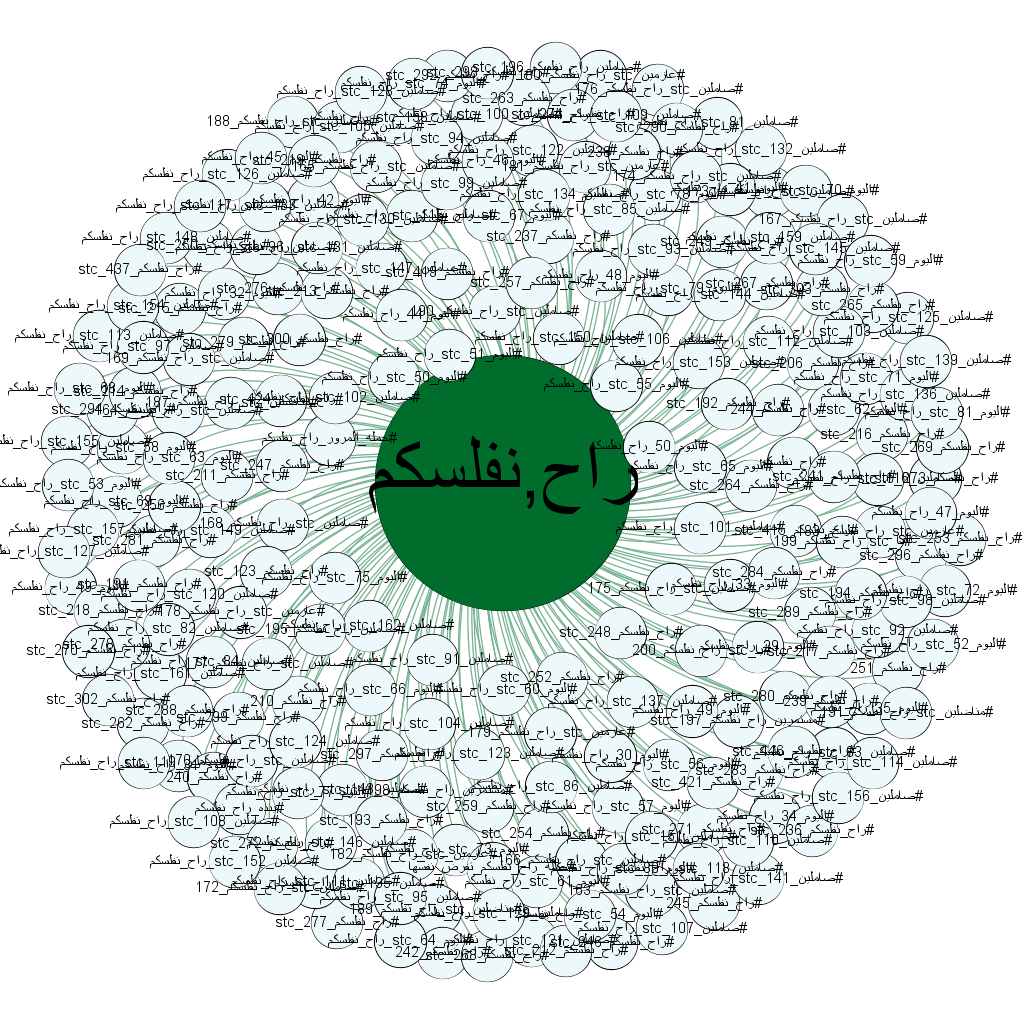
\includegraphics[width=0.7\textwidth]{images/stc_chain.png}
\caption{Topic chain for STC boycott trends}
\label{fig:stc_chain}
\end{figure*}

\subsection{Merging graphs: Country-Trend-Ngram}

Chain and tree graphs can be extended to provide more insights on participation of countries. Since the example in Figure~\ref{fig:ministers_tree} is relatively low in size, its visual representation will be clearer to present here. The ngram-trends graph above was merged with related edges from the base graph (country-trend).  This has resulted in more detailed graph, by which visualisation became more informative, as can be seen in Figure~\ref{fig:ctn_graph} below. This graph inherits nodes and edges from the combined graphs (country-trend and trend-ngram). Therefore, it includes three types of nodes; country, trend, and ngram, and two kinds of directed edges; country-trend and trend-ngram. So, paths flow as country-trend-ngram. 

Because there is one ngram node only, one colour and fixed size are used to distinguish it (green). For country nodes, shades of red are used for weighted outdegree, while node size reflects outdegree. Whereas for trend nodes, purples shades are used for weighted indegree and size indicates indegree.

\begin{figure*}[htb] \centering
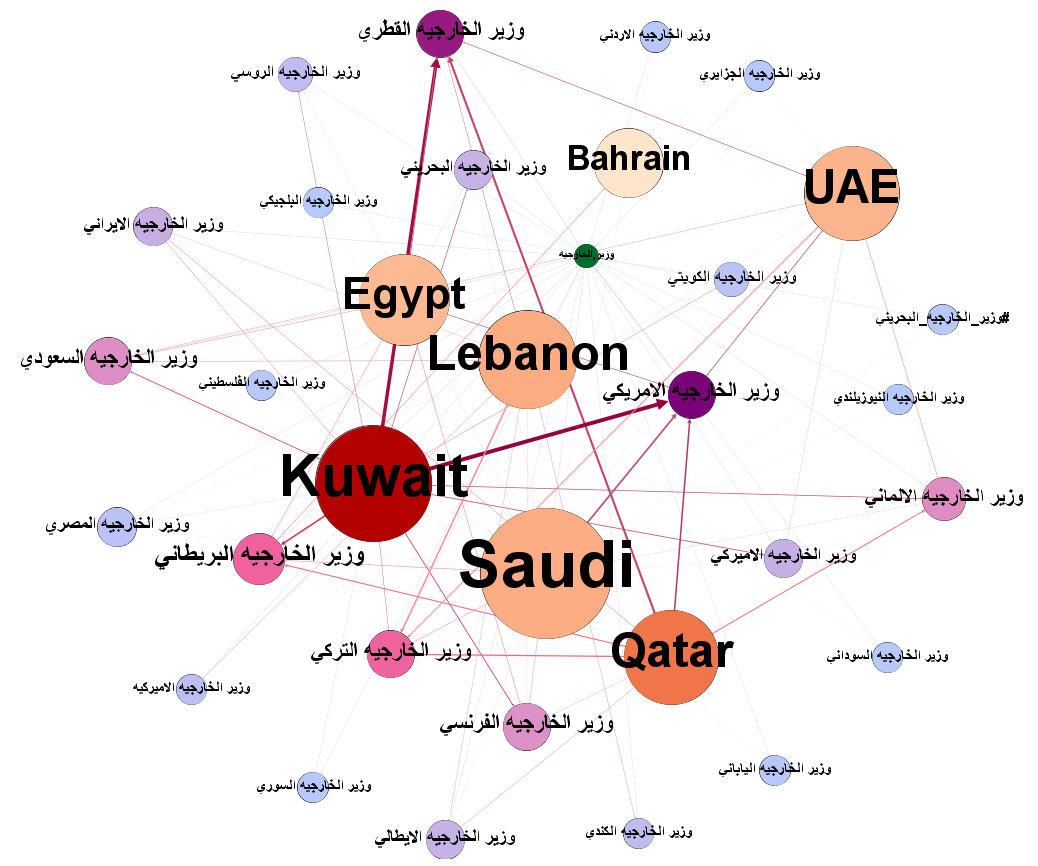
\includegraphics[width=0.7\textwidth]{images/ctn_graph.png}
\caption{Foreign ministers tree merged with weighed country-trend graph}
\label{fig:ctn_graph}
\end{figure*}

\section{Discussions}\label{discussion}

The analysis of trends showed a high repetitiveness in the more general trends, such as ‘\#good\_morning’, ‘\#Friday’, and ‘\#Trump’. Nevertheless, the topic ngrams helped to group the trends to provide a broader view. The trend-ngram graph facilitated the measurement of various forms of related trends.  For example, the bigram (‘We will, bankrupt you,’) was found in relation to 232 trends. As ngrams are inclusive, the general graphs favoured smaller ngrams, such as unigrams and bigrams, over larger forms. Therefore, the ngram-specific graphs were more useful in conducting a more accurate analysis, and could be tailored, based on the breadth of analysis required.  For example, the trend-unigram graph helped to extract all of the trends relating to a specific word, while the trend-trigram graph provided a more specific view of a topic.  Meanwhile, using the chain likelihood measure in the trend-ngram graph helped to identify certain important topics and their graph structures. Although many related trends had chain likelihood values between 0 and 1, some important topics emerged in the perfect form of chains or trees, 0 for trees, or 1 for chains.  The longest chain was found to be the Arabic version of (Saudi\_women\_request\_guardianship\_omission), which had links to 224 trend versions. Trend chains were useful for identifying frequently trending topics, and reflected a good degree of organisation in promoting and running social media campaigns. Furthermore, the trend trees graph structures helped to identify the subtopics of related trends, and their root topic. In addition to the tree example in Figure~\ref{fig:ministers_tree}, the bigram (‘international\_day’) was found to be linked to 64 trends representing different celebrated days on Twitter. Other perfect forms of trees included matches for football clubs, such as (‘Real\_madrid’), and celebrity birthdays (‘birthday’).  The overall view of the chains and trees was that the trend chains possessed a consistent textual structure that constituted a form of tweeting consensus over time, and therefore increased the likelihood of further similar trends appearing in the chain. 


Nevertheless, the continuity and length of the chain is depended on other factors, such as real-world developments. In contrast, the trend trees were generic, and did not include a textual pattern, apart from containing the root ngram.  Therefore, for a social media campaigns that included a continuous trend generation, or trend chain, it is important to maintain a consistent chain textual pattern. Accordingly, branching a chain in terms of turning chains into trees, disturbed their consistency, and would engender a dispersed tweeting effort, hence lowering the chance of long chains.  This highlighted a vulnerability that might be exploited as a countermeasure, the existence of which might be observed in anti-government and boycott campaigns. Although this claim was not testified in this present study, a suggestion for future analysis would be to measure the temporal changes of the graph structures, and the chain likelihood value.  


\section{Conclusions}\label{conclusions}

This paper presented a mixed approach for trend analysis using graph construction and ngram textual analysis. The techniques were tested on one-year’s worth of trend data for seven Middle Eastern Arabic-speaking countries. The analysis of the data employed one temporal base graphs, and two derived graphs.  First, a directed base graph was generated to capture the country-trend relationships. For the trend nodes in this graph, other information, such as timestamp, was added as node attributes. This graph was used to measure trend popularity and the participation of the sample countries. From this graph, ngrams were generated from the trends to construct another directed base graph. The nodes in this graph represented trends and ngrams, and edges were created based on the trend-ngram relationships. The main attribute of these nodes was their word length, which was used to identify the chains and trees in the trends. Although the results showed perfect chain and tree structures, other mixed forms of structures could also be identified. For example, a tree of chains might be identified to provide another perspective of the results. Third, two graphs were combined to generate another directed graph, capturing both the country-trend, and trend-ngram relationships. Although the example shown was a perfect tree, this graph could be used to observe the contribution of countries in chains, or any other topic of interest. 

Finally, the visual representation of the graphs was produced in two forms. First, due to their size, graphs such as country-trend, and trend-ngram required filtering, which was applied to include the important nodes, their edges, and related nodes, based on their centrality measures. Some examples visualised included the top 10\% of nodes with a high-weighted indegree. 

The last form of visualisation was based on the node of interest. The example in Figure~\ref{fig:ministers_tree} were produced for hand-picked nodes, while the core node of the graph shown in Figure~\ref{fig:ctn_graph} was selected, and the related edges and nodes were then extracted before visualising the whole graph.  In conclusion, the approach presented can employed to measure broad public concerns, and prolonged matters, as well as the possible spread of trends, based on their historical records as well as their originating country. The flexibility of this approach means it is appropriate for the aim of analysis.  A real-time application of this approach would be useful for observing certain trend activities, such as studying trend data in order to capture trends relating to a predefined ngram for a particular group of countries, or to discover emerging trend chains or trees.


% \section{Additional Requirements}

% For additional requirements for specific article types and further information please refer to \href{http://www.frontiersin.org/about/AuthorGuidelines#AdditionalRequirements}{Author Guidelines}.

\section*{Conflict of Interest Statement}
%All financial, commercial or other relationships that might be perceived by the academic community as representing a potential conflict of interest must be disclosed. If no such relationship exists, authors will be asked to confirm the following statement: 

The authors declare that the research was conducted in the absence of any commercial or financial relationships that could be construed as a potential conflict of interest.

\section*{Author Contributions}
% The Author Contributions section is mandatory for all articles, including articles by sole authors. If an appropriate statement is not provided on submission, a standard one will be inserted during the production process. The Author Contributions statement must describe the contributions of individual authors referred to by their initials and, in doing so, all authors agree to be accountable for the content of the work. Please see  \href{http://home.frontiersin.org/about/author-guidelines#AuthorandContributors}{here} for full authorship criteria.

% \section*{Funding}
% Details of all funding sources should be provided, including grant numbers if applicable. Please ensure to add all necessary funding information, as after publication this is no longer possible.

% \section*{Acknowledgments}
% This is a short text to acknowledge the contributions of specific colleagues, institutions, or agencies that aided the efforts of the authors.

% \section*{Supplemental Data}
%  \href{http://home.frontiersin.org/about/author-guidelines#SupplementaryMaterial}{Supplementary Material} should be uploaded separately on submission, if there are Supplementary Figures, please include the caption in the same file as the figure. LaTeX Supplementary Material templates can be found in the Frontiers LaTeX folder.

% \section*{Data Availability Statement}
% The datasets [GENERATED/ANALYZED] for this study can be found in the [NAME OF REPOSITORY] [LINK].
% Please see the availability of data guidelines for more information, at https://www.frontiersin.org/about/author-guidelines#AvailabilityofData

\bibliographystyle{frontiersinSCNS_ENG_HUMS} % for Science, Engineering and Humanities and Social Sciences articles, for Humanities and Social Sciences articles please include page numbers in the in-text citations
%\bibliographystyle{frontiersinHLTH&FPHY} % for Health, Physics and Mathematics articles
\bibliography{frontiers2018}

\end{document}
